\documentclass[tikz,border=8pt]{standalone}
\usepackage{amsmath}
\usepackage{amssymb}
\usetikzlibrary{arrows.meta,positioning,fit,calc}

\begin{document}
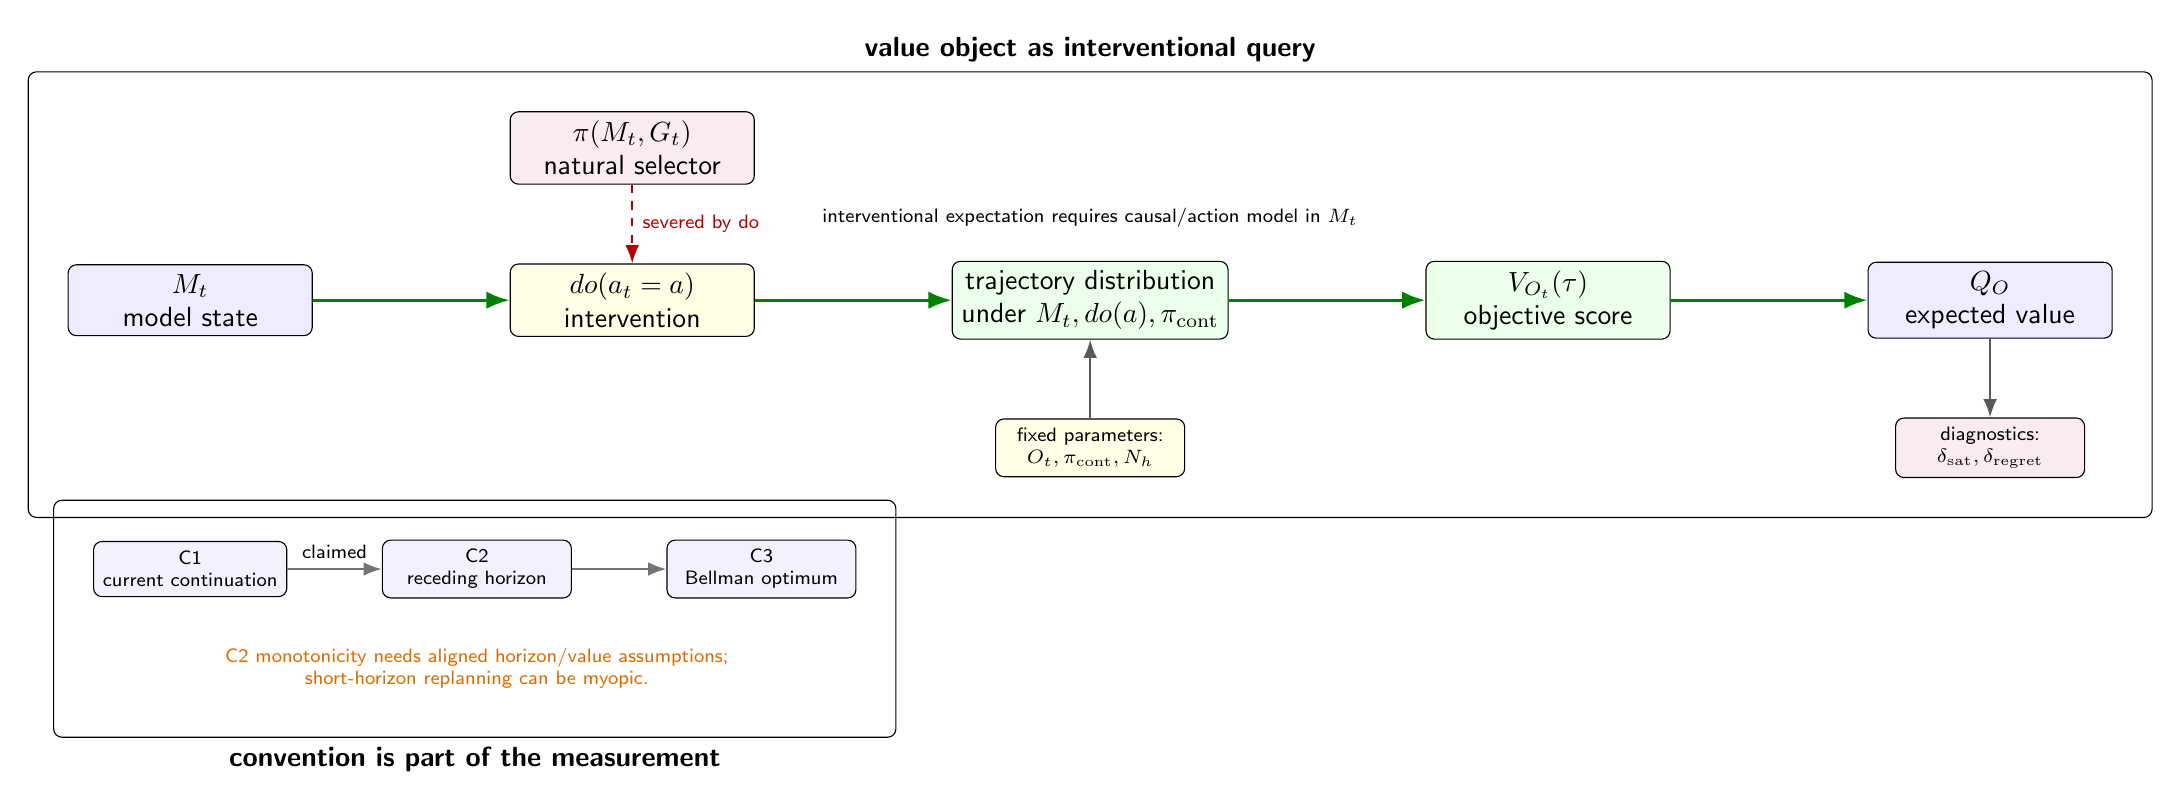
\begin{tikzpicture}[
  font=\sffamily,
  box/.style={draw, rounded corners=3pt, align=center, minimum width=31mm, minimum height=9mm, fill=white},
  small/.style={draw, rounded corners=3pt, align=center, minimum width=24mm, minimum height=7mm, fill=white, font=\sffamily\scriptsize},
  arrow/.style={-Latex, thick, draw=black!65},
  good/.style={-Latex, very thick, draw=green!50!black},
  cut/.style={-Latex, thick, dashed, draw=red!70!black},
  note/.style={align=center, font=\sffamily\scriptsize}
]

\node[box, fill=blue!7] (m) {$M_t$\\model state};
\node[box, right=25mm of m, fill=yellow!10] (doa) {$do(a_t=a)$\\intervention};
\node[box, above=10mm of doa, fill=purple!8] (nat) {$\pi(M_t,G_t)$\\natural selector};
\node[box, right=25mm of doa, fill=green!8] (dist) {trajectory distribution\\under $M_t,do(a),\pi_{\rm cont}$};
\node[box, right=25mm of dist, fill=green!8] (score) {$V_{O_t}(\tau)$\\objective score};
\node[box, right=25mm of score, fill=blue!7] (q) {$Q_O$\\expected value};

\node[small, below=10mm of dist, fill=yellow!10] (params) {fixed parameters:\\$O_t,\pi_{\rm cont},N_h$};
\node[small, below=10mm of q, fill=purple!8] (diag) {diagnostics:\\$\delta_{\rm sat},\delta_{\rm regret}$};

\draw[good] (m) -- (doa);
\draw[good] (doa) -- (dist);
\draw[good] (dist) -- (score);
\draw[good] (score) -- (q);
\draw[arrow] (params) -- (dist);
\draw[arrow] (q) -- (diag);

\draw[cut] (nat) -- node[right, note, text=red!70!black] {severed by do} (doa);
\node[note, above=3mm of dist] {interventional expectation requires causal/action model in $M_t$};

\node[small, below=26mm of m, fill=blue!5] (c1) {C1\\current continuation};
\node[small, right=12mm of c1, fill=blue!5] (c2) {C2\\receding horizon};
\node[small, right=12mm of c2, fill=blue!5] (c3) {C3\\Bellman optimum};
\draw[-Latex, thick, draw=black!55] (c1) -- node[above, note] {claimed} (c2);
\draw[-Latex, thick, draw=black!55] (c2) -- (c3);
\node[note, below=5mm of c2, text=orange!85!black] (warn)
  {C2 monotonicity needs aligned horizon/value assumptions;\\short-horizon replanning can be myopic.};

\node[draw, rounded corners=3pt, fit=(m)(doa)(dist)(score)(q)(params)(diag)(nat), inner sep=5mm,
  label={[font=\sffamily\bfseries]above:value object as interventional query}] {};
\node[draw, rounded corners=3pt, fit=(c1)(c2)(c3)(warn), inner sep=5mm,
  label={[font=\sffamily\bfseries]below:convention is part of the measurement}] {};

\end{tikzpicture}
\end{document}
